\chapter{BMO: un entorno aislado donde utilizar machine learning} \label{chap:4}

\vspace*{5mm}

\section{Introducción} \label{sec:4.1}

\emph{BMO}, personaje de la serie de televisión \emph{Hora de Aventuras} (figura \ref{fig:4.1}\footnote{Fuente de la imagen: \url{http://adventuretime.wikia.com/wiki/BMO}}), es un pequeño robot inteligente que aprende constantemente observando y participando en el mundo vivo que le rodea.

\begin{figure}[ht]
  \centering
  
\includegraphics[width=50mm]{figures/ch_04/bmo_adventure_time.png}
  \caption{BMO, personaje de la serie de televisión Hora de Aventuras.}
  \label{fig:4.1}
\end{figure}

Siendo el machine learning parte fundamental de la \emph{Inteligencia Artificial}, no encontré mejor nombre para una posible herramienta que me permitiera utilizar lo aprendido de aprendizaje automático de forma simple y rápida. Este herramienta, o conjunto de ellas, debía satisfacer varios requisitos, que para mí, eran indispensables dada la manera en la que trabajo con mis equipos informáticos:

\begin{itemize}
\item[\textbullet] Poseer una instalación sencilla, y en pocos pasos, para no encontrar problemas durante el proceso en equipos nuevos o recién \emph{limpios}.

\item[\textbullet] El entorno de la herramienta debe estar aislado, para no encontrar conflictos, incluso futuros, con otras herramientas instaladas de propósito general u otros objetivos específicos como el desarrollo.

\item[\textbullet] Poder ampliar la herramienta con cualquier aplicación o paquete necesario.

\item[\textbullet] Acceder al entorno de la herramienta desde la web para poder monitorizar o corregir imprevistos desde cualquier lugar.
\end{itemize}

Estos requisitos sesgaban bastante el rango de herramientas individuales a elegir. La decisión final fue que BMO envolviera de forma sencilla a {IPython Notebook} con los paquetes \emph{Python} necesarios para trabajar con machine learning, apoyándose en Docker para aislarlo del resto de software que se encuentra en el sistema operativo. En las siguientes secciones veremos el por qué de esta elección.

\section{Python frente a R} \label{sec:4.2}

A la hora de buscar herramientas para utilizar machine learning necesitaba que éstas fueran librerías para lenguajes de programación, y no herramientas auto-guiadas (con interfaz gráfica o no), para así poder aprovechar el potencial que ofrecen, como por ejemplo, usar varias de ellas a la vez o poder realizar pequeños cambios en su código. Además, debía buscar lenguajes fáciles de usar, ya que al fin y al cabo, los resultados que obtuviera serían nada más que prototipos, teniendo que buscar soluciones súper eficientes y solamente dedicadas a un problema en concreto si los quería usar en sistemas reales, algo más costoso en tiempo.

Con una simple búsqueda en Google como "\emph{programming languages for machine learning}", se pueden encontrar entradas en blogs y foros dedicados a machine learning y \emph{data science}, término que se ha puesto de moda en 2012, donde son tres los lenguajes que más se repiten: R, Python y Julia.

Eliminando a \emph{Julia}, ya que le falta madurar y ampliar su conjunto de librerías, elegir entre Python y R no fue fácil. Siendo \emph{R} un lenguaje creado para estadística computacional posee una sintaxis bastante idónea para las matemáticas, incluso es bastante eficiente para estas tareas, teniendo en cuenta que es un lenguaje interpretado. Además, lo acompañan estupendas librerías de alta calidad para poner en práctica todo tipo de algoritmos y métodos de aprendizaje automático. Finalmente, R posee un estupendo IDE para tareas científicas llamado RStudio, el cual puede ejecutarse desde el escritorio o la web.

En cambio, \emph{Python} es un lenguaje de propósito general, con una sintaxis tan simple y clara que parece pseudocódigo escrito en inglés. El principal problema de Python es su rendimiento, el habitual que se puede encontrar en un lenguaje interpretado. Para paliar esto, posee estupendas librerías de ámbito científico y para machine learning, donde el núcleo de casi todas están escrito en C, consiguiendo una gran mejora en el rendimiento. Al contrario que R, Python no posee IDE propio, pero no le faltan externos. Los más interesantes en el ámbito científico y académico son Spyder, muy parecido a RStudio pero sin poseer interfaz web, e IPython Notebook. Esté último no es un IDE, sino un entorno \emph{REPL}\footnote{REPL son las siglas de \emph{read-eval-print loop}, \emph{bucle de lectura-evaluación-impresión} en español.} para la web donde, además de poder visualizar las salidas de las sentencias Python, incluidas imágenes (figura \ref{fig:4.2}), tenemos funciones más complejas como el autocompletado de código. Uno de sus puntos fuertes es la inclusión, mediante extensiones, de más lenguajes, como el mismo R o Haskell.

\begin{figure}[H]
  \centering
  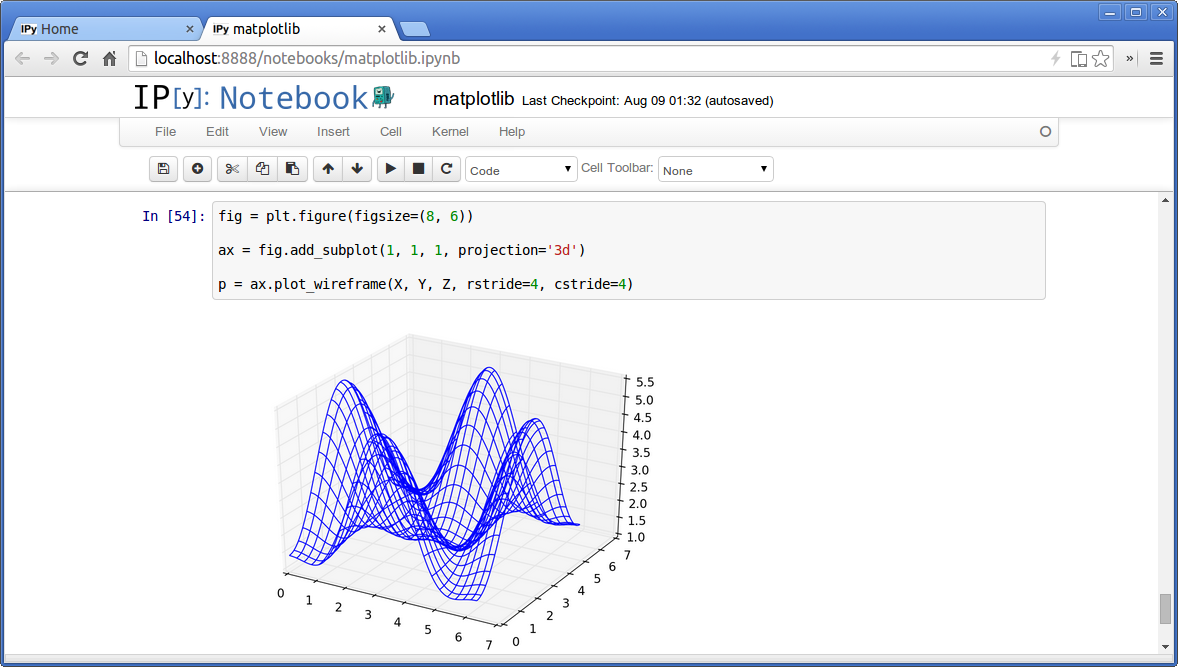
\includegraphics[width=130mm]{figures/ch_04/ipython_notebook.png}
  \caption{Notebook de IPython Notebook donde se practica con \emph{matplotlib}, una de las librerías de plotting para Python.}
  \label{fig:4.2}
\end{figure}

Aunque cada uno tiene su lugar en el ámbito de machine learning, decidí utilizar Python por su carácter como lenguaje de propósito general. Además en diferentes medios se empieza a hablar de cómo Python está desplazando a R como lenguaje para el data science\footnote{Una de estas múltiples opiniones la podemos encontrar en \emph{ReadWrite}: \url{http://readwr.it/a2CB}}. Por último, la versatilidad de IPython Notebook fue el último ingrediente de esta decisión.

\section{Docker frente a Vagrant} \label{sec:4.3}

Uno de los requisitos que necesitaba para BMO era que la herramienta fuera un entorno aislado, donde las aplicaciones y sus paquetes no interfirieran con los del sistema operativo y viceversa. La solución más simple era usar una máquina virtual, pero dado su alto consumo en recursos de la máquina anfitriona era una de las últimas opciones. Además, el gran tamaño físico de una máquina virtual junto a un conjunto de herramientas de machine learning, hacía pesada su distribución, por lo que una herramienta de automatización como Puppet\footnote{\url{http://puppetlabs.com/}} o Chef\footnote{\url{http://www.getchef.com/}}, o una exclusiva para máquinas virtuales como \emph{Vagrant}\footnote{\url{https://www.vagrantup.com/}}, era casi indispensable. Pero la solución llegó por parte de un proyecto open source, \emph{Docker}\footnote{\url{https://www.docker.com/}}.

Docker es un herramienta completamente similar a Vagrant, ofreciendo automatización y gestión de entornos, pero en lugar de máquinas virtuales, gestiona \emph{contenedores Linux}. Un contenedor no es nada más que un espacio en la memoria del sistema operativo donde se ejecutan procesos de manera completamente aislada, solamente pudiendo salir del entorno ciertas acciones del proceso si están permitidas explícitamente, como por ejemplo la escritura en disco. Su comportamiento general es como tener un pequeño sistema Linux dentro de una instalación Linux normal, con la ventaja de que apenas consume recursos. Pero su gran limitación está ahí, sólo funcionan en entornos Linux. Este problema realmente no lo es tanto por unos de lo requerimientos, acceder a BMO desde la web, dado que el uso de Linux para servidores web es mayoritario en la red\footnote{Según el medio W3Techs casi alcanzan el 40\% del total: \url{http://en.wikipedia.org/wiki/Usage_share_of_operating_systems\#Servers_on_the_Internet}}, sobre todo en ámbitos científicos.

Usando Docker, BMO se puede descargar rápidamente al solo ocupar $1GB$, o también se puede construir automáticamente en algo más de tiempo, debido a la compilación de ciertas herramientas.

\section{Herramientas instaladas} \label{sec:4.4}

Al ser BMO un pequeño entorno Linux, se puede añadir cualquier aplicación o paquete que resulte necesario, cumpliendo el último requisito que faltaba. Pero por defecto, BMO incluye los siguientes paquetes Python instalados:

\begin{description}
\item[beautifulsoup4] Parseador de documentos HTML.

\item[gensim] Modelador estadístico de temáticas para textos.

\item[matplotlib] Librería de plotting totalmente configurable.

\item[networkx] Librería de análisis de grafos y redes.

\item[nltk] Conjunto de librerías para procesamiento simbólico y estadístico de lenguaje natural.

\item[numpy] Extensión de Python para ofrecer soporte y funciones a grandes matrices multidimensionales.

\item[patsy] Librería para describir modelos estadísticos.

\item[pandas] Librería de manipulación y análisis simple de datos.

\item[pattern] Conjuntos de librerías de web mining.

\item[scikit-learn] Librería de machine learning para Python. Es la más extendida y madura de las disponibles.

\item[scipy] Conjunto de algoritmos y herramientas matemáticas para fines científicos.

\item[simpy] Librería para la simulación de eventos.
\end{description}

Además, en la sección \nameref{sec:a.2} del apéndice \ref{chap:ap_a}, podemos encontrar el apartado \emph{Examples and tutorials}, con una selección de ejemplos y tutoriales para IPython Notebook y para algunas de estas librerías, todos ellos creados por la comunidad de Python.

\section{Comparación con otras herramientas} \label{sec:4.5}

¿Por qué crear BMO y no usar una herramienta existente? Para responder a esta pregunta, la tabla \ref{table:4.1} ofrece una comparativa de las herramientas que ya existían, comparándolas con BMO.

\begin{table}[H]
\begin{adjustwidth}{-20mm}{-20mm}
\centering
\colorbox{lightgray}{\begin{tabular}{*{5}{c}}
  & \textbf{Entorno} & \textbf{Cloud} & \textbf{Python} & \textbf{R} \\
  \textbf{Data Science Toolbox} & Vagrant & Soportados por Vagrant & Si & Si \\
  \textbf{Data Science Box} & Ninguno & Amazon & Si & Si \\
  \textbf{Ŷhat Sciencebox} & Ninguno & Amazon & Si & Si \\
  \textbf{BMO} & Docker & Cualquiera con Docker & Si & No
\end{tabular}}
\caption{Comparación de herramientas de machine learning.}
\label{table:4.1}
\end{adjustwidth}
\end{table}

Lo que más puede llamar la atención es que BMO no lleva instalado R, aunque es extremadamente fácil de instalar en este entorno. En un segundo vistazo a la tabla se puede observar que algunas de las herramientas \emph{sólo} se pueden instalar en la nube, Data Science Box\footnote{\url{https://github.com/drewconway/data_science_box}} y Ŷhat Sciencebox\footnote{\url{https://github.com/drewconway/data_science_box}}, y la que no sin contar BMO, Data Science Toolbox\footnote{\url{https://github.com/DataScienceToolbox/data-science-toolbox/}}, usa máquinas virtuales a través de Vagrant, algo que se descartó al encontrar Docker.

\section{Conclusiones} \label{sec:4.6}

Por supuesto, BMO no es la herramienta perfecta ya que se pueden mejorar algunas de sus características para aumentar el número y mejorar sus casos de uso. Una de estas mejoras ya se ha comentado, la inclusión de R y sus herramientas. Otra característica a incluir puede ser alguna librería de procesamiento de imágenes. El motivo por el que no se ha incluido ninguna es que existe un gran número de librerías para esto propósito, por lo que lo más probable es que ninguna satisfaga las necesidades, o el simple gusto, de todo posible usuario. De todas formas, esto no supone un gran problema, ya que cualquiera de estas librerías se puede instalar sin problemas.

Para finalizar, decir que tras haber usado BMO para el caso práctico del capítulo \ref{chap:5} y en mi trabajo, he podido comprobar su utilizad tanto por su fácil instalación, sin ningún problema en varios equipos, y su aislamiento a la hora de trabajar, ya que se instaló en máquinas que ya contaban con grandes entornos Python. Por útlimo, como se comenta en el apéndice \ref{chap:ap_a}, BMO está disponible en \href{https://github.com/josemazo/bmo}{GitHub} liberado bajo \emph{licencia MIT}.
